\documentclass[1p]{elsarticle_modified}
%\bibliographystyle{elsarticle-num}

%\usepackage[colorlinks]{hyperref}
%\usepackage{abbrmath_seonhwa} %\Abb, \Ascr, \Acal ,\Abf, \Afrak
\usepackage{amsfonts}
\usepackage{amssymb}
\usepackage{amsmath}
\usepackage{amsthm}
\usepackage{scalefnt}
\usepackage{amsbsy}
\usepackage{kotex}
\usepackage{caption}
\usepackage{subfig}
\usepackage{color}
\usepackage{graphicx}
\usepackage{xcolor} %% white, black, red, green, blue, cyan, magenta, yellow
\usepackage{float}
\usepackage{setspace}
\usepackage{hyperref}

\usepackage{tikz}
\usetikzlibrary{arrows}

\usepackage{multirow}
\usepackage{array} % fixed length table
\usepackage{hhline}

%%%%%%%%%%%%%%%%%%%%%
\makeatletter
\renewcommand*\env@matrix[1][\arraystretch]{%
	\edef\arraystretch{#1}%
	\hskip -\arraycolsep
	\let\@ifnextchar\new@ifnextchar
	\array{*\c@MaxMatrixCols c}}
\makeatother %https://tex.stackexchange.com/questions/14071/how-can-i-increase-the-line-spacing-in-a-matrix
%%%%%%%%%%%%%%%

\usepackage[normalem]{ulem}

\newcommand{\msout}[1]{\ifmmode\text{\sout{\ensuremath{#1}}}\else\sout{#1}\fi}
%SOURCE: \msout is \stkout macro in https://tex.stackexchange.com/questions/20609/strikeout-in-math-mode

\newcommand{\cancel}[1]{
	\ifmmode
	{\color{red}\msout{#1}}
	\else
	{\color{red}\sout{#1}}
	\fi
}

\newcommand{\add}[1]{
	{\color{blue}\uwave{#1}}
}

\newcommand{\replace}[2]{
	\ifmmode
	{\color{red}\msout{#1}}{\color{blue}\uwave{#2}}
	\else
	{\color{red}\sout{#1}}{\color{blue}\uwave{#2}}
	\fi
}

\newcommand{\Sol}{\mathcal{S}} %segment
\newcommand{\D}{D} %diagram
\newcommand{\A}{\mathcal{A}} %arc


%%%%%%%%%%%%%%%%%%%%%%%%%%%%%5 test

\def\sl{\operatorname{\textup{SL}}(2,\Cbb)}
\def\psl{\operatorname{\textup{PSL}}(2,\Cbb)}
\def\quan{\mkern 1mu \triangleright \mkern 1mu}

\theoremstyle{definition}
\newtheorem{thm}{Theorem}[section]
\newtheorem{prop}[thm]{Proposition}
\newtheorem{lem}[thm]{Lemma}
\newtheorem{ques}[thm]{Question}
\newtheorem{cor}[thm]{Corollary}
\newtheorem{defn}[thm]{Definition}
\newtheorem{exam}[thm]{Example}
\newtheorem{rmk}[thm]{Remark}
\newtheorem{alg}[thm]{Algorithm}

\newcommand{\I}{\sqrt{-1}}
\begin{document}

%\begin{frontmatter}
%
%\title{Boundary parabolic representations of knots up to 8 crossings}
%
%%% Group authors per affiliation:
%\author{Yunhi Cho} 
%\address{Department of Mathematics, University of Seoul, Seoul, Korea}
%\ead{yhcho@uos.ac.kr}
%
%
%\author{Seonhwa Kim} %\fnref{s_kim}}
%\address{Center for Geometry and Physics, Institute for Basic Science, Pohang, 37673, Korea}
%\ead{ryeona17@ibs.re.kr}
%
%\author{Hyuk Kim}
%\address{Department of Mathematical Sciences, Seoul National University, Seoul 08826, Korea}
%\ead{hyukkim@snu.ac.kr}
%
%\author{Seokbeom Yoon}
%\address{Department of Mathematical Sciences, Seoul National University, Seoul, 08826,  Korea}
%\ead{sbyoon15@snu.ac.kr}
%
%\begin{abstract}
%We find all boundary parabolic representation of knots up to 8 crossings.
%
%\end{abstract}
%\begin{keyword}
%    \MSC[2010] 57M25 
%\end{keyword}
%
%\end{frontmatter}

%\linenumbers
%\tableofcontents
%
\newcommand\colored[1]{\textcolor{white}{\rule[-0.35ex]{0.8em}{1.4ex}}\kern-0.8em\color{red} #1}%
%\newcommand\colored[1]{\textcolor{white}{ #1}\kern-2.17ex	\textcolor{white}{ #1}\kern-1.81ex	\textcolor{white}{ #1}\kern-2.15ex\color{red}#1	}

{\Large $\underline{12n_{0384}~(K12n_{0384})}$}

\setlength{\tabcolsep}{10pt}
\renewcommand{\arraystretch}{1.6}
\vspace{1cm}\begin{tabular}{m{100pt}>{\centering\arraybackslash}m{274pt}}
\multirow{5}{120pt}{
	\centering
	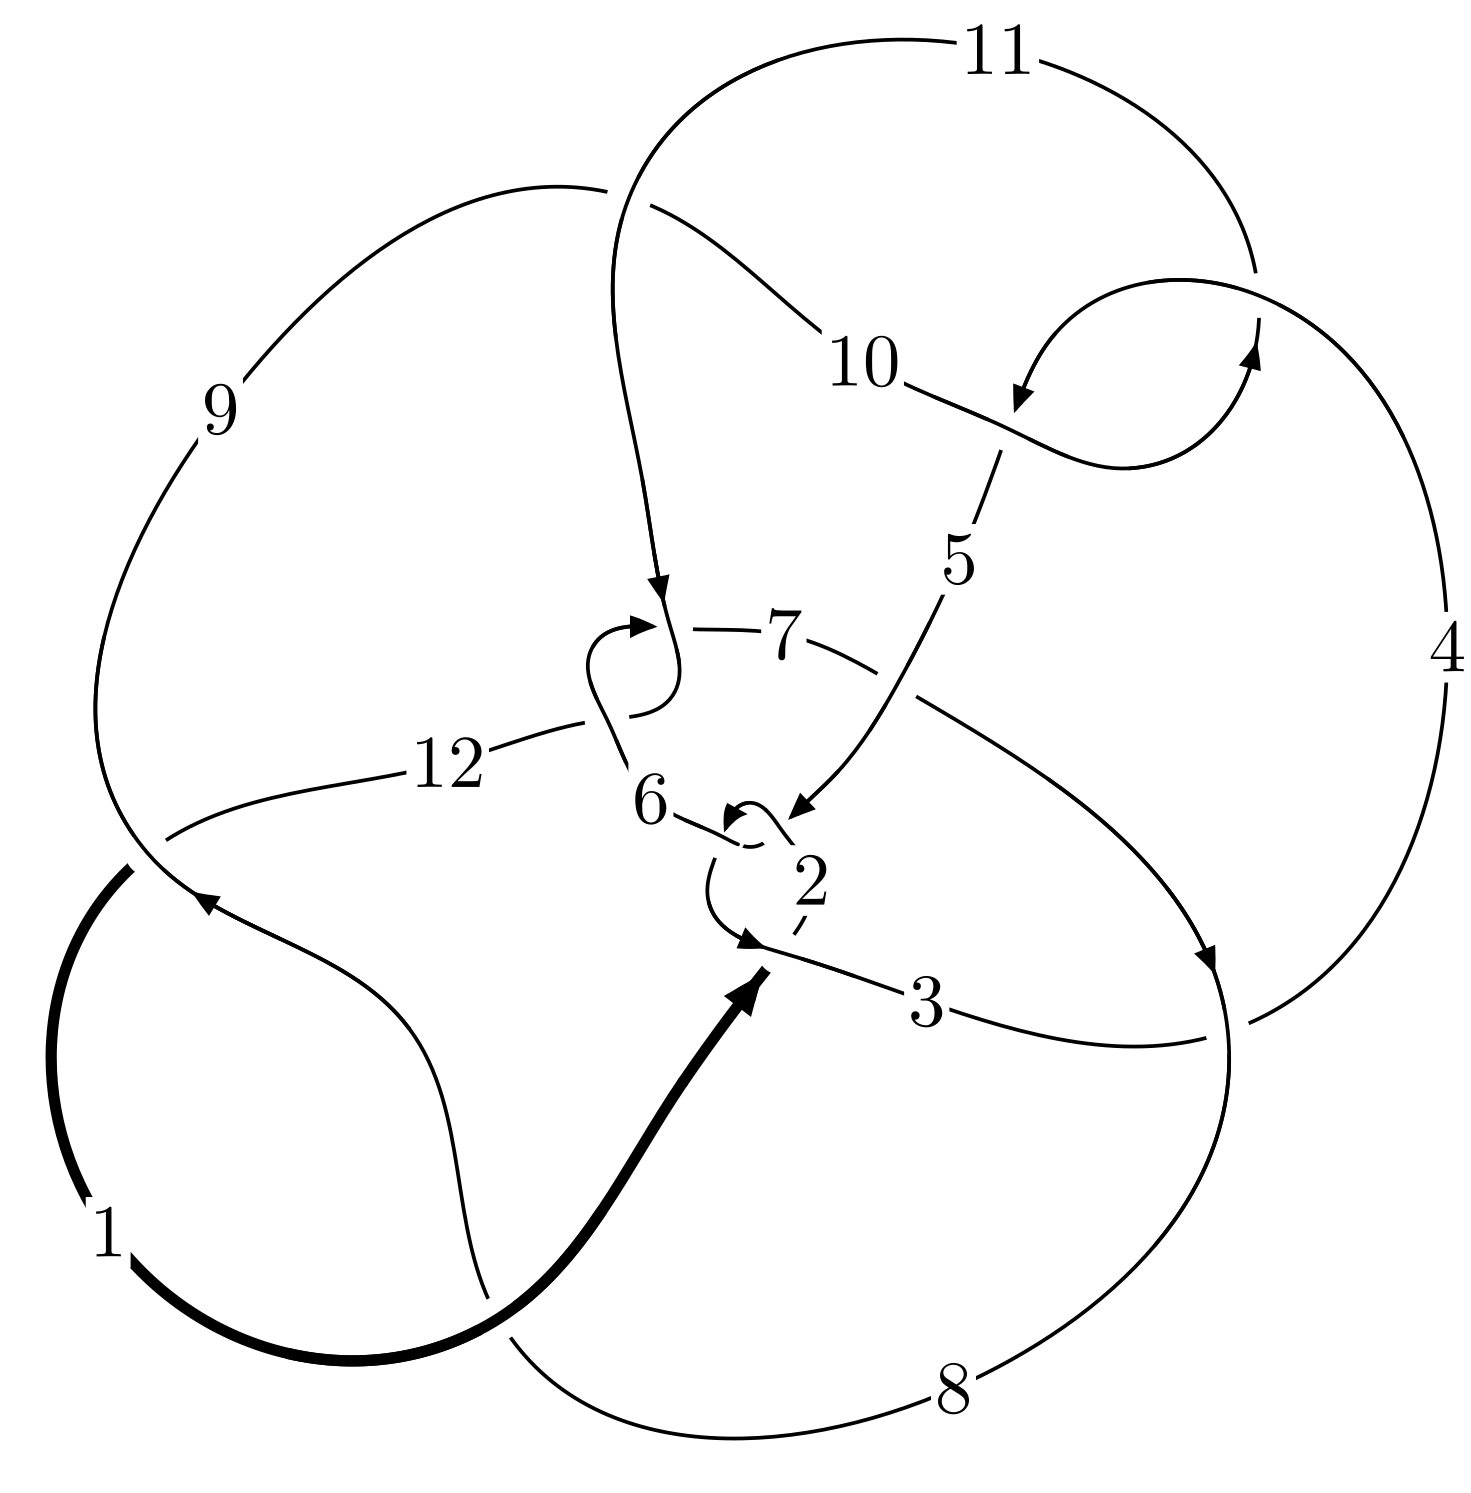
\includegraphics[width=112pt]{../../../GIT/diagram.site/Diagrams/png/2473_12n_0384.png}\\
\ \ \ A knot diagram\footnotemark}&
\allowdisplaybreaks
\textbf{Linearized knot diagam} \\
\cline{2-2}
 &
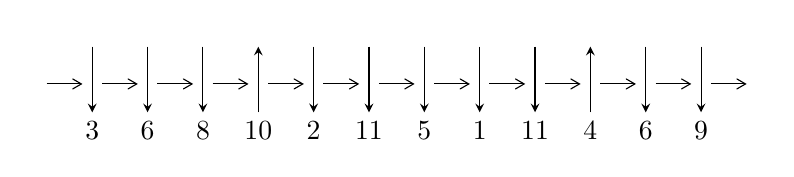
\begin{tikzpicture}[x=20pt, y=17pt]
	% nodes
	\node (C0) at (0, 0) {};
	\node (C1) at (1, 0) {};
	\node (C1U) at (1, +1) {};
	\node (C1D) at (1, -1) {3};

	\node (C2) at (2, 0) {};
	\node (C2U) at (2, +1) {};
	\node (C2D) at (2, -1) {6};

	\node (C3) at (3, 0) {};
	\node (C3U) at (3, +1) {};
	\node (C3D) at (3, -1) {8};

	\node (C4) at (4, 0) {};
	\node (C4U) at (4, +1) {};
	\node (C4D) at (4, -1) {10};

	\node (C5) at (5, 0) {};
	\node (C5U) at (5, +1) {};
	\node (C5D) at (5, -1) {2};

	\node (C6) at (6, 0) {};
	\node (C6U) at (6, +1) {};
	\node (C6D) at (6, -1) {11};

	\node (C7) at (7, 0) {};
	\node (C7U) at (7, +1) {};
	\node (C7D) at (7, -1) {5};

	\node (C8) at (8, 0) {};
	\node (C8U) at (8, +1) {};
	\node (C8D) at (8, -1) {1};

	\node (C9) at (9, 0) {};
	\node (C9U) at (9, +1) {};
	\node (C9D) at (9, -1) {11};

	\node (C10) at (10, 0) {};
	\node (C10U) at (10, +1) {};
	\node (C10D) at (10, -1) {4};

	\node (C11) at (11, 0) {};
	\node (C11U) at (11, +1) {};
	\node (C11D) at (11, -1) {6};

	\node (C12) at (12, 0) {};
	\node (C12U) at (12, +1) {};
	\node (C12D) at (12, -1) {9};
	\node (C13) at (13, 0) {};

	% arrows
	\draw[->,>={angle 60}]
	(C0) edge (C1) (C1) edge (C2) (C2) edge (C3) (C3) edge (C4) (C4) edge (C5) (C5) edge (C6) (C6) edge (C7) (C7) edge (C8) (C8) edge (C9) (C9) edge (C10) (C10) edge (C11) (C11) edge (C12) (C12) edge (C13) ;	\draw[->,>=stealth]
	(C1U) edge (C1D) (C2U) edge (C2D) (C3U) edge (C3D) (C4D) edge (C4U) (C5U) edge (C5D) (C6U) edge (C6D) (C7U) edge (C7D) (C8U) edge (C8D) (C9U) edge (C9D) (C10D) edge (C10U) (C11U) edge (C11D) (C12U) edge (C12D) ;
	\end{tikzpicture} \\
\hhline{~~} \\& 
\textbf{Solving Sequence} \\ \cline{2-2} 
 &
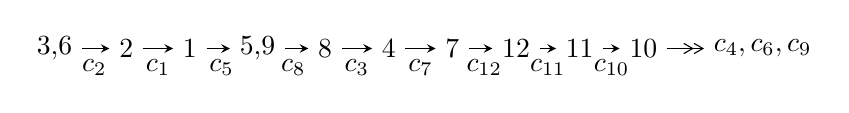
\begin{tikzpicture}[x=23pt, y=7pt]
	% node
	\node (A0) at (-1/8, 0) {3,6};
	\node (A1) at (1, 0) {2};
	\node (A2) at (2, 0) {1};
	\node (A3) at (49/16, 0) {5,9};
	\node (A4) at (33/8, 0) {8};
	\node (A5) at (41/8, 0) {4};
	\node (A6) at (49/8, 0) {7};
	\node (A7) at (57/8, 0) {12};
	\node (A8) at (65/8, 0) {11};
	\node (A9) at (73/8, 0) {10};
	\node (C1) at (1/2, -1) {$c_{2}$};
	\node (C2) at (3/2, -1) {$c_{1}$};
	\node (C3) at (5/2, -1) {$c_{5}$};
	\node (C4) at (29/8, -1) {$c_{8}$};
	\node (C5) at (37/8, -1) {$c_{3}$};
	\node (C6) at (45/8, -1) {$c_{7}$};
	\node (C7) at (53/8, -1) {$c_{12}$};
	\node (C8) at (61/8, -1) {$c_{11}$};
	\node (C9) at (69/8, -1) {$c_{10}$};
	\node (A10) at (11, 0) {$c_{4},c_{6},c_{9}$};

	% edge
	\draw[->,>=stealth]	
	(A0) edge (A1) (A1) edge (A2) (A2) edge (A3) (A3) edge (A4) (A4) edge (A5) (A5) edge (A6) (A6) edge (A7) (A7) edge (A8) (A8) edge (A9) ;
	\draw[->>,>={angle 60}]	
	(A9) edge (A10);
\end{tikzpicture} \\ 

\end{tabular} \\

\footnotetext{
The image of knot diagram is generated by the software ``\textbf{Draw programme}" developed by Andrew Bartholomew(\url{http://www.layer8.co.uk/maths/draw/index.htm\#Running-draw}), where we modified some parts for our purpose(\url{https://github.com/CATsTAILs/LinksPainter}).
}\phantom \\ \newline 
\centering \textbf{Ideals for irreducible components\footnotemark of $X_{\text{par}}$} 
 
\begin{align*}
I^u_{1}&=\langle 
-2.71603\times10^{130} u^{78}-3.34605\times10^{130} u^{77}+\cdots+9.47150\times10^{129} b-1.79777\times10^{130},\\
\phantom{I^u_{1}}&\phantom{= \langle  }-2.58758\times10^{129} u^{78}-1.91076\times10^{130} u^{77}+\cdots+9.47150\times10^{129} a-5.72706\times10^{130},\\
\phantom{I^u_{1}}&\phantom{= \langle  }u^{79}+2 u^{78}+\cdots+3 u+1\rangle \\
I^u_{2}&=\langle 
- u^{22}+6 u^{20}+\cdots+b+1,\;6 u^{22}+5 u^{21}+\cdots+a-7,\;u^{23}+u^{22}+\cdots- u-1\rangle \\
\\
\end{align*}
\raggedright * 2 irreducible components of $\dim_{\mathbb{C}}=0$, with total 102 representations.\\
\footnotetext{All coefficients of polynomials are rational numbers. But the coefficients are sometimes approximated in decimal forms when there is not enough margin.}
\newpage
\renewcommand{\arraystretch}{1}
\centering \section*{I. $I^u_{1}= \langle -2.72\times10^{130} u^{78}-3.35\times10^{130} u^{77}+\cdots+9.47\times10^{129} b-1.80\times10^{130},\;-2.59\times10^{129} u^{78}-1.91\times10^{130} u^{77}+\cdots+9.47\times10^{129} a-5.73\times10^{130},\;u^{79}+2 u^{78}+\cdots+3 u+1 \rangle$}
\flushleft \textbf{(i) Arc colorings}\\
\begin{tabular}{m{7pt} m{180pt} m{7pt} m{180pt} }
\flushright $a_{3}=$&$\begin{pmatrix}1\\0\end{pmatrix}$ \\
\flushright $a_{6}=$&$\begin{pmatrix}0\\u\end{pmatrix}$ \\
\flushright $a_{2}=$&$\begin{pmatrix}1\\- u^2\end{pmatrix}$ \\
\flushright $a_{1}=$&$\begin{pmatrix}- u^2+1\\- u^2\end{pmatrix}$ \\
\flushright $a_{5}=$&$\begin{pmatrix}u\\- u^3+u\end{pmatrix}$ \\
\flushright $a_{9}=$&$\begin{pmatrix}0.273197 u^{78}+2.01738 u^{77}+\cdots-9.55208 u+6.04662\\2.86758 u^{78}+3.53276 u^{77}+\cdots+10.8984 u+1.89808\end{pmatrix}$ \\
\flushright $a_{8}=$&$\begin{pmatrix}-0.309986 u^{78}+0.455035 u^{77}+\cdots-9.66549 u+3.32245\\2.02383 u^{78}+2.39814 u^{77}+\cdots+8.31238 u+0.949213\end{pmatrix}$ \\
\flushright $a_{4}=$&$\begin{pmatrix}-1.71680 u^{78}-3.26582 u^{77}+\cdots-2.40110 u-5.06109\\-2.85920 u^{78}-4.22104 u^{77}+\cdots-9.93888 u-4.06187\end{pmatrix}$ \\
\flushright $a_{7}=$&$\begin{pmatrix}1.43940 u^{78}+3.19611 u^{77}+\cdots-3.75783 u+5.82097\\3.55209 u^{78}+4.65508 u^{77}+\cdots+13.6963 u+2.69004\end{pmatrix}$ \\
\flushright $a_{12}=$&$\begin{pmatrix}1.08140 u^{78}+2.11225 u^{77}+\cdots+8.48887 u+6.87053\\3.83910 u^{78}+5.49216 u^{77}+\cdots+10.2711 u+4.75553\end{pmatrix}$ \\
\flushright $a_{11}=$&$\begin{pmatrix}1.08140 u^{78}+2.11225 u^{77}+\cdots+8.48887 u+6.87053\\3.86348 u^{78}+5.61449 u^{77}+\cdots+11.2009 u+4.70499\end{pmatrix}$ \\
\flushright $a_{10}=$&$\begin{pmatrix}3.04438 u^{78}+6.01782 u^{77}+\cdots-3.93386 u+5.29498\\0.834964 u^{78}+1.28035 u^{77}+\cdots+7.27458 u+2.68116\end{pmatrix}$\\&\end{tabular}
\flushleft \textbf{(ii) Obstruction class $= -1$}\\~\\
\flushleft \textbf{(iii) Cusp Shapes $= 1.45357 u^{78}+4.69764 u^{77}+\cdots-16.7472 u-8.13507$}\\~\\
\newpage\renewcommand{\arraystretch}{1}
\flushleft \textbf{(iv) u-Polynomials at the component}\newline \\
\begin{tabular}{m{50pt}|m{274pt}}
Crossings & \hspace{64pt}u-Polynomials at each crossing \\
\hline $$\begin{aligned}c_{1}\end{aligned}$$&$\begin{aligned}
&u^{79}+40 u^{78}+\cdots+33 u+1
\end{aligned}$\\
\hline $$\begin{aligned}c_{2},c_{5}\end{aligned}$$&$\begin{aligned}
&u^{79}+2 u^{78}+\cdots+3 u+1
\end{aligned}$\\
\hline $$\begin{aligned}c_{3}\end{aligned}$$&$\begin{aligned}
&u^{79}+u^{78}+\cdots+3042 u+1971
\end{aligned}$\\
\hline $$\begin{aligned}c_{4},c_{10}\end{aligned}$$&$\begin{aligned}
&u^{79}+u^{78}+\cdots+6 u^2+1
\end{aligned}$\\
\hline $$\begin{aligned}c_{6},c_{11}\end{aligned}$$&$\begin{aligned}
&u^{79}+2 u^{78}+\cdots+33033 u+2741
\end{aligned}$\\
\hline $$\begin{aligned}c_{7}\end{aligned}$$&$\begin{aligned}
&u^{79}- u^{78}+\cdots-15955220 u+4890941
\end{aligned}$\\
\hline $$\begin{aligned}c_{8},c_{12}\end{aligned}$$&$\begin{aligned}
&u^{79}-4 u^{78}+\cdots+465 u-71
\end{aligned}$\\
\hline $$\begin{aligned}c_{9}\end{aligned}$$&$\begin{aligned}
&u^{79}+45 u^{78}+\cdots-12 u-1
\end{aligned}$\\
\hline
\end{tabular}\\~\\
\newpage\renewcommand{\arraystretch}{1}
\flushleft \textbf{(v) Riley Polynomials at the component}\newline \\
\begin{tabular}{m{50pt}|m{274pt}}
Crossings & \hspace{64pt}Riley Polynomials at each crossing \\
\hline $$\begin{aligned}c_{1}\end{aligned}$$&$\begin{aligned}
&y^{79}+12 y^{78}+\cdots-27 y-1
\end{aligned}$\\
\hline $$\begin{aligned}c_{2},c_{5}\end{aligned}$$&$\begin{aligned}
&y^{79}-40 y^{78}+\cdots+33 y-1
\end{aligned}$\\
\hline $$\begin{aligned}c_{3}\end{aligned}$$&$\begin{aligned}
&y^{79}+41 y^{78}+\cdots-122003010 y-3884841
\end{aligned}$\\
\hline $$\begin{aligned}c_{4},c_{10}\end{aligned}$$&$\begin{aligned}
&y^{79}+45 y^{78}+\cdots-12 y-1
\end{aligned}$\\
\hline $$\begin{aligned}c_{6},c_{11}\end{aligned}$$&$\begin{aligned}
&y^{79}-62 y^{78}+\cdots-310804037 y-7513081
\end{aligned}$\\
\hline $$\begin{aligned}c_{7}\end{aligned}$$&$\begin{aligned}
&y^{79}-43 y^{78}+\cdots+243479110423596 y-23921303865481
\end{aligned}$\\
\hline $$\begin{aligned}c_{8},c_{12}\end{aligned}$$&$\begin{aligned}
&y^{79}+30 y^{78}+\cdots+195635 y-5041
\end{aligned}$\\
\hline $$\begin{aligned}c_{9}\end{aligned}$$&$\begin{aligned}
&y^{79}-11 y^{78}+\cdots+72 y-1
\end{aligned}$\\
\hline
\end{tabular}\\~\\
\newpage\flushleft \textbf{(vi) Complex Volumes and Cusp Shapes}
$$\begin{array}{c|c|c}  
\text{Solutions to }I^u_{1}& \I (\text{vol} + \sqrt{-1}CS) & \text{Cusp shape}\\
 \hline 
\begin{aligned}
u &= -0.191031 + 0.984252 I \\
a &= -0.07978 - 1.48636 I \\
b &= \phantom{-}0.508156 - 0.260237 I\end{aligned}
 & -3.18307 - 0.81586 I & \phantom{-0.000000 } 0 \\ \hline\begin{aligned}
u &= -0.191031 - 0.984252 I \\
a &= -0.07978 + 1.48636 I \\
b &= \phantom{-}0.508156 + 0.260237 I\end{aligned}
 & -3.18307 + 0.81586 I & \phantom{-0.000000 } 0 \\ \hline\begin{aligned}
u &= \phantom{-}0.772897 + 0.639352 I \\
a &= \phantom{-}1.62485 - 0.20199 I \\
b &= \phantom{-}1.47815 - 1.36105 I\end{aligned}
 & \phantom{-}3.37009 - 0.55634 I & \phantom{-0.000000 } 0 \\ \hline\begin{aligned}
u &= \phantom{-}0.772897 - 0.639352 I \\
a &= \phantom{-}1.62485 + 0.20199 I \\
b &= \phantom{-}1.47815 + 1.36105 I\end{aligned}
 & \phantom{-}3.37009 + 0.55634 I & \phantom{-0.000000 } 0 \\ \hline\begin{aligned}
u &= \phantom{-}0.279781 + 0.946093 I \\
a &= \phantom{-}0.422327 - 0.009943 I \\
b &= \phantom{-}0.387992 - 0.507427 I\end{aligned}
 & \phantom{-}4.25236 - 1.51303 I & \phantom{-0.000000 } 0 \\ \hline\begin{aligned}
u &= \phantom{-}0.279781 - 0.946093 I \\
a &= \phantom{-}0.422327 + 0.009943 I \\
b &= \phantom{-}0.387992 + 0.507427 I\end{aligned}
 & \phantom{-}4.25236 + 1.51303 I & \phantom{-0.000000 } 0 \\ \hline\begin{aligned}
u &= \phantom{-}0.347049 + 0.957087 I \\
a &= -0.13702 - 1.41951 I \\
b &= -0.865084 - 0.221243 I\end{aligned}
 & \phantom{-}1.35913 + 5.11137 I & \phantom{-0.000000 } 0 \\ \hline\begin{aligned}
u &= \phantom{-}0.347049 - 0.957087 I \\
a &= -0.13702 + 1.41951 I \\
b &= -0.865084 + 0.221243 I\end{aligned}
 & \phantom{-}1.35913 - 5.11137 I & \phantom{-0.000000 } 0 \\ \hline\begin{aligned}
u &= -0.949703 + 0.369866 I \\
a &= -1.071130 - 0.249125 I \\
b &= \phantom{-}0.195225 - 0.520375 I\end{aligned}
 & \phantom{-}1.207890 + 0.693296 I & \phantom{-0.000000 } 0 \\ \hline\begin{aligned}
u &= -0.949703 - 0.369866 I \\
a &= -1.071130 + 0.249125 I \\
b &= \phantom{-}0.195225 + 0.520375 I\end{aligned}
 & \phantom{-}1.207890 - 0.693296 I & \phantom{-0.000000 } 0\\
 \hline 
 \end{array}$$\newpage$$\begin{array}{c|c|c}  
\text{Solutions to }I^u_{1}& \I (\text{vol} + \sqrt{-1}CS) & \text{Cusp shape}\\
 \hline 
\begin{aligned}
u &= \phantom{-}0.651752 + 0.803645 I \\
a &= \phantom{-}1.028100 + 0.127820 I \\
b &= \phantom{-}1.080790 - 0.665746 I\end{aligned}
 & \phantom{-}3.75206 - 1.01538 I & \phantom{-0.000000 } 0 \\ \hline\begin{aligned}
u &= \phantom{-}0.651752 - 0.803645 I \\
a &= \phantom{-}1.028100 - 0.127820 I \\
b &= \phantom{-}1.080790 + 0.665746 I\end{aligned}
 & \phantom{-}3.75206 + 1.01538 I & \phantom{-0.000000 } 0 \\ \hline\begin{aligned}
u &= -0.735451 + 0.763114 I \\
a &= -1.33628 + 0.71471 I \\
b &= -1.65988 - 0.43120 I\end{aligned}
 & \phantom{-}1.52896 - 1.89063 I & \phantom{-0.000000 } 0 \\ \hline\begin{aligned}
u &= -0.735451 - 0.763114 I \\
a &= -1.33628 - 0.71471 I \\
b &= -1.65988 + 0.43120 I\end{aligned}
 & \phantom{-}1.52896 + 1.89063 I & \phantom{-0.000000 } 0 \\ \hline\begin{aligned}
u &= -0.390500 + 1.044200 I \\
a &= \phantom{-}0.23951 - 1.54767 I \\
b &= \phantom{-}0.954518 - 0.436619 I\end{aligned}
 & -1.91185 - 10.39900 I & \phantom{-0.000000 } 0 \\ \hline\begin{aligned}
u &= -0.390500 - 1.044200 I \\
a &= \phantom{-}0.23951 + 1.54767 I \\
b &= \phantom{-}0.954518 + 0.436619 I\end{aligned}
 & -1.91185 + 10.39900 I & \phantom{-0.000000 } 0 \\ \hline\begin{aligned}
u &= \phantom{-}1.110500 + 0.123199 I \\
a &= -0.360738 - 0.519588 I \\
b &= \phantom{-}0.355883 - 0.926772 I\end{aligned}
 & -4.60003 - 2.24012 I & \phantom{-0.000000 } 0 \\ \hline\begin{aligned}
u &= \phantom{-}1.110500 - 0.123199 I \\
a &= -0.360738 + 0.519588 I \\
b &= \phantom{-}0.355883 + 0.926772 I\end{aligned}
 & -4.60003 + 2.24012 I & \phantom{-0.000000 } 0 \\ \hline\begin{aligned}
u &= \phantom{-}1.032050 + 0.440550 I \\
a &= -1.155910 + 0.517509 I \\
b &= -1.324490 + 0.224798 I\end{aligned}
 & -3.64519 - 2.75689 I & \phantom{-0.000000 } 0 \\ \hline\begin{aligned}
u &= \phantom{-}1.032050 - 0.440550 I \\
a &= -1.155910 - 0.517509 I \\
b &= -1.324490 - 0.224798 I\end{aligned}
 & -3.64519 + 2.75689 I & \phantom{-0.000000 } 0\\
 \hline 
 \end{array}$$\newpage$$\begin{array}{c|c|c}  
\text{Solutions to }I^u_{1}& \I (\text{vol} + \sqrt{-1}CS) & \text{Cusp shape}\\
 \hline 
\begin{aligned}
u &= -0.799671 + 0.338631 I \\
a &= -1.32453 - 0.80993 I \\
b &= -0.78022 - 2.11425 I\end{aligned}
 & \phantom{-}1.77333 + 2.34825 I & -10.56329 - 4.52984 I \\ \hline\begin{aligned}
u &= -0.799671 - 0.338631 I \\
a &= -1.32453 + 0.80993 I \\
b &= -0.78022 + 2.11425 I\end{aligned}
 & \phantom{-}1.77333 - 2.34825 I & -10.56329 + 4.52984 I \\ \hline\begin{aligned}
u &= \phantom{-}1.075170 + 0.388500 I \\
a &= -0.949388 + 0.662897 I \\
b &= -1.49346 + 2.56287 I\end{aligned}
 & -7.23041 + 1.32092 I & \phantom{-0.000000 } 0 \\ \hline\begin{aligned}
u &= \phantom{-}1.075170 - 0.388500 I \\
a &= -0.949388 - 0.662897 I \\
b &= -1.49346 - 2.56287 I\end{aligned}
 & -7.23041 - 1.32092 I & \phantom{-0.000000 } 0 \\ \hline\begin{aligned}
u &= \phantom{-}0.983798 + 0.587300 I \\
a &= \phantom{-}0.261400 - 0.889339 I \\
b &= -0.878215 - 0.255984 I\end{aligned}
 & \phantom{-}2.69035 - 4.34043 I & \phantom{-0.000000 } 0 \\ \hline\begin{aligned}
u &= \phantom{-}0.983798 - 0.587300 I \\
a &= \phantom{-}0.261400 + 0.889339 I \\
b &= -0.878215 + 0.255984 I\end{aligned}
 & \phantom{-}2.69035 + 4.34043 I & \phantom{-0.000000 } 0 \\ \hline\begin{aligned}
u &= -1.047200 + 0.470329 I \\
a &= \phantom{-}1.121370 + 0.298241 I \\
b &= \phantom{-}1.64342 + 2.17778 I\end{aligned}
 & -3.40305 + 3.75556 I & \phantom{-0.000000 } 0 \\ \hline\begin{aligned}
u &= -1.047200 - 0.470329 I \\
a &= \phantom{-}1.121370 - 0.298241 I \\
b &= \phantom{-}1.64342 - 2.17778 I\end{aligned}
 & -3.40305 - 3.75556 I & \phantom{-0.000000 } 0 \\ \hline\begin{aligned}
u &= -1.062590 + 0.466582 I \\
a &= -0.473431 - 0.104262 I \\
b &= -1.77680 - 0.79310 I\end{aligned}
 & \phantom{-}3.25715 + 0.42701 I & \phantom{-0.000000 } 0 \\ \hline\begin{aligned}
u &= -1.062590 - 0.466582 I \\
a &= -0.473431 + 0.104262 I \\
b &= -1.77680 + 0.79310 I\end{aligned}
 & \phantom{-}3.25715 - 0.42701 I & \phantom{-0.000000 } 0\\
 \hline 
 \end{array}$$\newpage$$\begin{array}{c|c|c}  
\text{Solutions to }I^u_{1}& \I (\text{vol} + \sqrt{-1}CS) & \text{Cusp shape}\\
 \hline 
\begin{aligned}
u &= \phantom{-}0.979155 + 0.659990 I \\
a &= -0.186768 - 1.044480 I \\
b &= -1.192080 - 0.090654 I\end{aligned}
 & \phantom{-}2.67066 - 4.41905 I & \phantom{-0.000000 } 0 \\ \hline\begin{aligned}
u &= \phantom{-}0.979155 - 0.659990 I \\
a &= -0.186768 + 1.044480 I \\
b &= -1.192080 + 0.090654 I\end{aligned}
 & \phantom{-}2.67066 + 4.41905 I & \phantom{-0.000000 } 0 \\ \hline\begin{aligned}
u &= -1.068830 + 0.513419 I \\
a &= \phantom{-}1.238950 + 0.404006 I \\
b &= \phantom{-}1.59996 + 0.25716 I\end{aligned}
 & -6.37531 + 8.24596 I & \phantom{-0.000000 } 0 \\ \hline\begin{aligned}
u &= -1.068830 - 0.513419 I \\
a &= \phantom{-}1.238950 - 0.404006 I \\
b &= \phantom{-}1.59996 - 0.25716 I\end{aligned}
 & -6.37531 - 8.24596 I & \phantom{-0.000000 } 0 \\ \hline\begin{aligned}
u &= \phantom{-}1.088050 + 0.498479 I \\
a &= \phantom{-}0.566854 - 0.120059 I \\
b &= \phantom{-}1.81501 - 1.09357 I\end{aligned}
 & \phantom{-}3.49995 - 6.66947 I & \phantom{-0.000000 } 0 \\ \hline\begin{aligned}
u &= \phantom{-}1.088050 - 0.498479 I \\
a &= \phantom{-}0.566854 + 0.120059 I \\
b &= \phantom{-}1.81501 + 1.09357 I\end{aligned}
 & \phantom{-}3.49995 + 6.66947 I & \phantom{-0.000000 } 0 \\ \hline\begin{aligned}
u &= -1.148050 + 0.354073 I \\
a &= \phantom{-}1.229620 + 0.676225 I \\
b &= \phantom{-}1.207310 + 0.678030 I\end{aligned}
 & -8.51556 - 0.93201 I & \phantom{-0.000000 } 0 \\ \hline\begin{aligned}
u &= -1.148050 - 0.354073 I \\
a &= \phantom{-}1.229620 - 0.676225 I \\
b &= \phantom{-}1.207310 - 0.678030 I\end{aligned}
 & -8.51556 + 0.93201 I & \phantom{-0.000000 } 0 \\ \hline\begin{aligned}
u &= -0.911687 + 0.787204 I \\
a &= \phantom{-}0.803246 - 0.640191 I \\
b &= \phantom{-}1.113530 + 0.554256 I\end{aligned}
 & \phantom{-}0.87775 + 2.17137 I & \phantom{-0.000000 } 0 \\ \hline\begin{aligned}
u &= -0.911687 - 0.787204 I \\
a &= \phantom{-}0.803246 + 0.640191 I \\
b &= \phantom{-}1.113530 - 0.554256 I\end{aligned}
 & \phantom{-}0.87775 - 2.17137 I & \phantom{-0.000000 } 0\\
 \hline 
 \end{array}$$\newpage$$\begin{array}{c|c|c}  
\text{Solutions to }I^u_{1}& \I (\text{vol} + \sqrt{-1}CS) & \text{Cusp shape}\\
 \hline 
\begin{aligned}
u &= -0.971228 + 0.714175 I \\
a &= \phantom{-}0.99212 - 1.26649 I \\
b &= \phantom{-}1.87985 + 0.21111 I\end{aligned}
 & \phantom{-}0.81093 + 7.49828 I & \phantom{-0.000000 } 0 \\ \hline\begin{aligned}
u &= -0.971228 - 0.714175 I \\
a &= \phantom{-}0.99212 + 1.26649 I \\
b &= \phantom{-}1.87985 - 0.21111 I\end{aligned}
 & \phantom{-}0.81093 - 7.49828 I & \phantom{-0.000000 } 0 \\ \hline\begin{aligned}
u &= -0.792183\phantom{ +0.000000I} \\
a &= \phantom{-}0.614293\phantom{ +0.000000I} \\
b &= -0.625628\phantom{ +0.000000I}\end{aligned}
 & -1.33059\phantom{ +0.000000I} & -6.58480\phantom{ +0.000000I} \\ \hline\begin{aligned}
u &= \phantom{-}1.107910 + 0.516873 I \\
a &= -1.50586 + 0.31421 I \\
b &= -2.06147 + 2.18423 I\end{aligned}
 & -7.42311 - 8.62365 I & \phantom{-0.000000 } 0 \\ \hline\begin{aligned}
u &= \phantom{-}1.107910 - 0.516873 I \\
a &= -1.50586 - 0.31421 I \\
b &= -2.06147 - 2.18423 I\end{aligned}
 & -7.42311 + 8.62365 I & \phantom{-0.000000 } 0 \\ \hline\begin{aligned}
u &= \phantom{-}0.715864 + 0.277463 I \\
a &= -1.46137 + 0.89491 I \\
b &= -0.541854 - 0.023836 I\end{aligned}
 & -2.22862 - 0.48454 I & -3.32397 + 5.38263 I \\ \hline\begin{aligned}
u &= \phantom{-}0.715864 - 0.277463 I \\
a &= -1.46137 - 0.89491 I \\
b &= -0.541854 + 0.023836 I\end{aligned}
 & -2.22862 + 0.48454 I & -3.32397 - 5.38263 I \\ \hline\begin{aligned}
u &= -0.833390 + 0.940010 I \\
a &= -0.894586 + 0.345537 I \\
b &= -1.165880 - 0.263330 I\end{aligned}
 & \phantom{-}1.16138 + 4.13478 I & \phantom{-0.000000 } 0 \\ \hline\begin{aligned}
u &= -0.833390 - 0.940010 I \\
a &= -0.894586 - 0.345537 I \\
b &= -1.165880 + 0.263330 I\end{aligned}
 & \phantom{-}1.16138 - 4.13478 I & \phantom{-0.000000 } 0 \\ \hline\begin{aligned}
u &= \phantom{-}1.192740 + 0.640609 I \\
a &= \phantom{-}1.142680 - 0.139516 I \\
b &= \phantom{-}1.93724 - 1.46494 I\end{aligned}
 & -1.21826 - 10.92240 I & \phantom{-0.000000 } 0\\
 \hline 
 \end{array}$$\newpage$$\begin{array}{c|c|c}  
\text{Solutions to }I^u_{1}& \I (\text{vol} + \sqrt{-1}CS) & \text{Cusp shape}\\
 \hline 
\begin{aligned}
u &= \phantom{-}1.192740 - 0.640609 I \\
a &= \phantom{-}1.142680 + 0.139516 I \\
b &= \phantom{-}1.93724 + 1.46494 I\end{aligned}
 & -1.21826 + 10.92240 I & \phantom{-0.000000 } 0 \\ \hline\begin{aligned}
u &= \phantom{-}1.109620 + 0.776023 I \\
a &= -0.529150 - 0.336994 I \\
b &= -0.961927 + 0.438116 I\end{aligned}
 & \phantom{-}2.08413 - 4.66431 I & \phantom{-0.000000 } 0 \\ \hline\begin{aligned}
u &= \phantom{-}1.109620 - 0.776023 I \\
a &= -0.529150 + 0.336994 I \\
b &= -0.961927 - 0.438116 I\end{aligned}
 & \phantom{-}2.08413 + 4.66431 I & \phantom{-0.000000 } 0 \\ \hline\begin{aligned}
u &= -0.454850 + 0.447099 I \\
a &= \phantom{-}1.39866 + 2.20652 I \\
b &= \phantom{-}0.339961 + 0.112299 I\end{aligned}
 & -4.50604 - 4.04932 I & -6.45793 + 1.67799 I \\ \hline\begin{aligned}
u &= -0.454850 - 0.447099 I \\
a &= \phantom{-}1.39866 - 2.20652 I \\
b &= \phantom{-}0.339961 - 0.112299 I\end{aligned}
 & -4.50604 + 4.04932 I & -6.45793 - 1.67799 I \\ \hline\begin{aligned}
u &= -1.237660 + 0.581931 I \\
a &= -1.042670 - 0.390086 I \\
b &= -1.81279 - 1.57352 I\end{aligned}
 & -6.38355 + 6.41792 I & \phantom{-0.000000 } 0 \\ \hline\begin{aligned}
u &= -1.237660 - 0.581931 I \\
a &= -1.042670 + 0.390086 I \\
b &= -1.81279 + 1.57352 I\end{aligned}
 & -6.38355 - 6.41792 I & \phantom{-0.000000 } 0 \\ \hline\begin{aligned}
u &= -0.564621 + 0.284535 I \\
a &= -0.545059 - 0.268663 I \\
b &= \phantom{-}0.72095 + 1.66387 I\end{aligned}
 & \phantom{-}5.05746 + 3.12388 I & -8.19578 + 0.26827 I \\ \hline\begin{aligned}
u &= -0.564621 - 0.284535 I \\
a &= -0.545059 + 0.268663 I \\
b &= \phantom{-}0.72095 - 1.66387 I\end{aligned}
 & \phantom{-}5.05746 - 3.12388 I & -8.19578 - 0.26827 I \\ \hline\begin{aligned}
u &= \phantom{-}0.421372 + 0.463446 I \\
a &= \phantom{-}0.337655 - 0.819391 I \\
b &= -0.827292 + 1.047940 I\end{aligned}
 & \phantom{-}5.53379 + 2.54054 I & -4.42930 - 5.76558 I\\
 \hline 
 \end{array}$$\newpage$$\begin{array}{c|c|c}  
\text{Solutions to }I^u_{1}& \I (\text{vol} + \sqrt{-1}CS) & \text{Cusp shape}\\
 \hline 
\begin{aligned}
u &= \phantom{-}0.421372 - 0.463446 I \\
a &= \phantom{-}0.337655 + 0.819391 I \\
b &= -0.827292 - 1.047940 I\end{aligned}
 & \phantom{-}5.53379 - 2.54054 I & -4.42930 + 5.76558 I \\ \hline\begin{aligned}
u &= -1.359440 + 0.212786 I \\
a &= -0.770916 - 0.399157 I \\
b &= -1.080790 - 0.207121 I\end{aligned}
 & -4.45616 - 1.31756 I & \phantom{-0.000000 } 0 \\ \hline\begin{aligned}
u &= -1.359440 - 0.212786 I \\
a &= -0.770916 + 0.399157 I \\
b &= -1.080790 + 0.207121 I\end{aligned}
 & -4.45616 + 1.31756 I & \phantom{-0.000000 } 0 \\ \hline\begin{aligned}
u &= -1.275420 + 0.546485 I \\
a &= -0.0739416 + 0.1149980 I \\
b &= \phantom{-}0.375729 + 0.413377 I\end{aligned}
 & -0.12238 + 6.61116 I & \phantom{-0.000000 } 0 \\ \hline\begin{aligned}
u &= -1.275420 - 0.546485 I \\
a &= -0.0739416 - 0.1149980 I \\
b &= \phantom{-}0.375729 - 0.413377 I\end{aligned}
 & -0.12238 - 6.61116 I & \phantom{-0.000000 } 0 \\ \hline\begin{aligned}
u &= -1.211040 + 0.682574 I \\
a &= -1.315290 - 0.111684 I \\
b &= -2.03346 - 1.47490 I\end{aligned}
 & -4.4575 + 16.6063 I & \phantom{-0.000000 } 0 \\ \hline\begin{aligned}
u &= -1.211040 - 0.682574 I \\
a &= -1.315290 + 0.111684 I \\
b &= -2.03346 + 1.47490 I\end{aligned}
 & -4.4575 - 16.6063 I & \phantom{-0.000000 } 0 \\ \hline\begin{aligned}
u &= \phantom{-}0.184918 + 0.538457 I \\
a &= -0.11921 + 3.12712 I \\
b &= \phantom{-}0.950595 + 0.446805 I\end{aligned}
 & -5.02903 + 4.28349 I & -8.27681 - 4.00164 I \\ \hline\begin{aligned}
u &= \phantom{-}0.184918 - 0.538457 I \\
a &= -0.11921 - 3.12712 I \\
b &= \phantom{-}0.950595 - 0.446805 I\end{aligned}
 & -5.02903 - 4.28349 I & -8.27681 + 4.00164 I \\ \hline\begin{aligned}
u &= \phantom{-}1.40099 + 0.34736 I \\
a &= \phantom{-}0.850459 - 0.324010 I \\
b &= \phantom{-}1.245410 - 0.267260 I\end{aligned}
 & -8.36209 - 3.89179 I & \phantom{-0.000000 } 0\\
 \hline 
 \end{array}$$\newpage$$\begin{array}{c|c|c}  
\text{Solutions to }I^u_{1}& \I (\text{vol} + \sqrt{-1}CS) & \text{Cusp shape}\\
 \hline 
\begin{aligned}
u &= \phantom{-}1.40099 - 0.34736 I \\
a &= \phantom{-}0.850459 + 0.324010 I \\
b &= \phantom{-}1.245410 + 0.267260 I\end{aligned}
 & -8.36209 + 3.89179 I & \phantom{-0.000000 } 0 \\ \hline\begin{aligned}
u &= \phantom{-}1.47172 + 0.12727 I \\
a &= \phantom{-}0.789184 - 0.491099 I \\
b &= \phantom{-}0.972773 - 0.381657 I\end{aligned}
 & -8.61435 + 6.30190 I & \phantom{-0.000000 } 0 \\ \hline\begin{aligned}
u &= \phantom{-}1.47172 - 0.12727 I \\
a &= \phantom{-}0.789184 + 0.491099 I \\
b &= \phantom{-}0.972773 + 0.381657 I\end{aligned}
 & -8.61435 - 6.30190 I & \phantom{-0.000000 } 0 \\ \hline\begin{aligned}
u &= -0.373652 + 0.265576 I \\
a &= \phantom{-}1.88378 + 1.55663 I \\
b &= -0.941910 + 0.210297 I\end{aligned}
 & -1.53987 - 0.04744 I & -5.18898 - 0.81135 I \\ \hline\begin{aligned}
u &= -0.373652 - 0.265576 I \\
a &= \phantom{-}1.88378 - 1.55663 I \\
b &= -0.941910 - 0.210297 I\end{aligned}
 & -1.53987 + 0.04744 I & -5.18898 + 0.81135 I \\ \hline\begin{aligned}
u &= -0.280943 + 0.315261 I \\
a &= \phantom{-}0.413918 - 0.655502 I \\
b &= -0.145072 + 0.373722 I\end{aligned}
 & -0.455090 + 0.991741 I & -7.13691 - 6.73727 I \\ \hline\begin{aligned}
u &= -0.280943 - 0.315261 I \\
a &= \phantom{-}0.413918 + 0.655502 I \\
b &= -0.145072 - 0.373722 I\end{aligned}
 & -0.455090 - 0.991741 I & -7.13691 + 6.73727 I \\ \hline\begin{aligned}
u &= \phantom{-}0.337723 + 0.070804 I \\
a &= -4.81881 - 0.75247 I \\
b &= \phantom{-}1.093010 + 0.305232 I\end{aligned}
 & -4.84439 - 4.25943 I & -6.45155 + 7.25445 I \\ \hline\begin{aligned}
u &= \phantom{-}0.337723 - 0.070804 I \\
a &= -4.81881 + 0.75247 I \\
b &= \phantom{-}1.093010 - 0.305232 I\end{aligned}
 & -4.84439 + 4.25943 I & -6.45155 - 7.25445 I\\
 \hline 
 \end{array}$$\newpage\newpage\renewcommand{\arraystretch}{1}
\centering \section*{II. $I^u_{2}= \langle - u^{22}+6 u^{20}+\cdots+b+1,\;6 u^{22}+5 u^{21}+\cdots+a-7,\;u^{23}+u^{22}+\cdots- u-1 \rangle$}
\flushleft \textbf{(i) Arc colorings}\\
\begin{tabular}{m{7pt} m{180pt} m{7pt} m{180pt} }
\flushright $a_{3}=$&$\begin{pmatrix}1\\0\end{pmatrix}$ \\
\flushright $a_{6}=$&$\begin{pmatrix}0\\u\end{pmatrix}$ \\
\flushright $a_{2}=$&$\begin{pmatrix}1\\- u^2\end{pmatrix}$ \\
\flushright $a_{1}=$&$\begin{pmatrix}- u^2+1\\- u^2\end{pmatrix}$ \\
\flushright $a_{5}=$&$\begin{pmatrix}u\\- u^3+u\end{pmatrix}$ \\
\flushright $a_{9}=$&$\begin{pmatrix}-6 u^{22}-5 u^{21}+\cdots-13 u+7\\u^{22}-6 u^{20}+\cdots+4 u-1\end{pmatrix}$ \\
\flushright $a_{8}=$&$\begin{pmatrix}-7 u^{22}-5 u^{21}+\cdots-13 u+8\\u^{22}+u^{21}+\cdots+5 u-1\end{pmatrix}$ \\
\flushright $a_{4}=$&$\begin{pmatrix}6 u^{22}+u^{21}+\cdots+6 u-13\\- u^{22}+7 u^{20}+\cdots- u+5\end{pmatrix}$ \\
\flushright $a_{7}=$&$\begin{pmatrix}-5 u^{22}-4 u^{21}+\cdots-9 u+6\\2 u^{22}+u^{21}+\cdots+8 u-2\end{pmatrix}$ \\
\flushright $a_{12}=$&$\begin{pmatrix}u^{22}-7 u^{20}+\cdots+u-6\\-3 u^{22}- u^{21}+\cdots- u+2\end{pmatrix}$ \\
\flushright $a_{11}=$&$\begin{pmatrix}u^{22}-7 u^{20}+\cdots+u-6\\-3 u^{22}- u^{21}+\cdots- u+3\end{pmatrix}$ \\
\flushright $a_{10}=$&$\begin{pmatrix}4 u^{22}-25 u^{20}+\cdots-4 u-8\\-4 u^{22}-2 u^{21}+\cdots-4 u+4\end{pmatrix}$\\&\end{tabular}
\flushleft \textbf{(ii) Obstruction class $= 1$}\\~\\
\flushleft \textbf{(iii) Cusp Shapes $= -5 u^{22}- u^{21}+29 u^{20}+10 u^{19}-87 u^{18}-44 u^{17}+168 u^{16}+116 u^{15}-205 u^{14}-199 u^{13}+147 u^{12}+231 u^{11}-22 u^{10}-175 u^9-78 u^8+88 u^7+89 u^6-23 u^5-82 u^4+u^3+34 u^2+6 u-21$}\\~\\
\newpage\renewcommand{\arraystretch}{1}
\flushleft \textbf{(iv) u-Polynomials at the component}\newline \\
\begin{tabular}{m{50pt}|m{274pt}}
Crossings & \hspace{64pt}u-Polynomials at each crossing \\
\hline $$\begin{aligned}c_{1}\end{aligned}$$&$\begin{aligned}
&u^{23}-13 u^{22}+\cdots+13 u-1
\end{aligned}$\\
\hline $$\begin{aligned}c_{2}\end{aligned}$$&$\begin{aligned}
&u^{23}+u^{22}+\cdots- u-1
\end{aligned}$\\
\hline $$\begin{aligned}c_{3}\end{aligned}$$&$\begin{aligned}
&u^{23}+10 u^{21}+\cdots-2 u+1
\end{aligned}$\\
\hline $$\begin{aligned}c_{4}\end{aligned}$$&$\begin{aligned}
&u^{23}+6 u^{21}+\cdots-2 u+1
\end{aligned}$\\
\hline $$\begin{aligned}c_{5}\end{aligned}$$&$\begin{aligned}
&u^{23}- u^{22}+\cdots- u+1
\end{aligned}$\\
\hline $$\begin{aligned}c_{6}\end{aligned}$$&$\begin{aligned}
&u^{23}+u^{22}+\cdots+3 u-1
\end{aligned}$\\
\hline $$\begin{aligned}c_{7}\end{aligned}$$&$\begin{aligned}
&u^{23}+8 u^{22}+\cdots+88 u-29
\end{aligned}$\\
\hline $$\begin{aligned}c_{8}\end{aligned}$$&$\begin{aligned}
&u^{23}-3 u^{22}+\cdots- u-1
\end{aligned}$\\
\hline $$\begin{aligned}c_{9}\end{aligned}$$&$\begin{aligned}
&u^{23}-12 u^{22}+\cdots-8 u+1
\end{aligned}$\\
\hline $$\begin{aligned}c_{10}\end{aligned}$$&$\begin{aligned}
&u^{23}+6 u^{21}+\cdots-2 u-1
\end{aligned}$\\
\hline $$\begin{aligned}c_{11}\end{aligned}$$&$\begin{aligned}
&u^{23}- u^{22}+\cdots+3 u+1
\end{aligned}$\\
\hline $$\begin{aligned}c_{12}\end{aligned}$$&$\begin{aligned}
&u^{23}+3 u^{22}+\cdots- u+1
\end{aligned}$\\
\hline
\end{tabular}\\~\\
\newpage\renewcommand{\arraystretch}{1}
\flushleft \textbf{(v) Riley Polynomials at the component}\newline \\
\begin{tabular}{m{50pt}|m{274pt}}
Crossings & \hspace{64pt}Riley Polynomials at each crossing \\
\hline $$\begin{aligned}c_{1}\end{aligned}$$&$\begin{aligned}
&y^{23}+7 y^{22}+\cdots+y-1
\end{aligned}$\\
\hline $$\begin{aligned}c_{2},c_{5}\end{aligned}$$&$\begin{aligned}
&y^{23}-13 y^{22}+\cdots+13 y-1
\end{aligned}$\\
\hline $$\begin{aligned}c_{3}\end{aligned}$$&$\begin{aligned}
&y^{23}+20 y^{22}+\cdots+10 y-1
\end{aligned}$\\
\hline $$\begin{aligned}c_{4},c_{10}\end{aligned}$$&$\begin{aligned}
&y^{23}+12 y^{22}+\cdots-8 y-1
\end{aligned}$\\
\hline $$\begin{aligned}c_{6},c_{11}\end{aligned}$$&$\begin{aligned}
&y^{23}-3 y^{22}+\cdots-13 y-1
\end{aligned}$\\
\hline $$\begin{aligned}c_{7}\end{aligned}$$&$\begin{aligned}
&y^{23}-4 y^{22}+\cdots+6932 y-841
\end{aligned}$\\
\hline $$\begin{aligned}c_{8},c_{12}\end{aligned}$$&$\begin{aligned}
&y^{23}+13 y^{22}+\cdots+3 y-1
\end{aligned}$\\
\hline $$\begin{aligned}c_{9}\end{aligned}$$&$\begin{aligned}
&y^{23}+8 y^{22}+\cdots-20 y-1
\end{aligned}$\\
\hline
\end{tabular}\\~\\
\newpage\flushleft \textbf{(vi) Complex Volumes and Cusp Shapes}
$$\begin{array}{c|c|c}  
\text{Solutions to }I^u_{2}& \I (\text{vol} + \sqrt{-1}CS) & \text{Cusp shape}\\
 \hline 
\begin{aligned}
u &= -0.630015 + 0.671543 I \\
a &= -1.101100 - 0.648550 I \\
b &= -0.787291 - 1.066420 I\end{aligned}
 & \phantom{-}3.03165 + 1.75887 I & -5.37226 - 4.25162 I \\ \hline\begin{aligned}
u &= -0.630015 - 0.671543 I \\
a &= -1.101100 + 0.648550 I \\
b &= -0.787291 + 1.066420 I\end{aligned}
 & \phantom{-}3.03165 - 1.75887 I & -5.37226 + 4.25162 I \\ \hline\begin{aligned}
u &= -0.703790 + 0.560880 I \\
a &= -0.759261 - 0.016715 I \\
b &= -1.48162 - 1.22442 I\end{aligned}
 & \phantom{-}5.66183 - 1.58895 I & -3.77306 - 1.87293 I \\ \hline\begin{aligned}
u &= -0.703790 - 0.560880 I \\
a &= -0.759261 + 0.016715 I \\
b &= -1.48162 + 1.22442 I\end{aligned}
 & \phantom{-}5.66183 + 1.58895 I & -3.77306 + 1.87293 I \\ \hline\begin{aligned}
u &= \phantom{-}0.683964 + 0.525529 I \\
a &= \phantom{-}0.834493 + 0.206624 I \\
b &= \phantom{-}1.36447 - 1.51147 I\end{aligned}
 & \phantom{-}5.48484 - 3.77860 I & -1.97875 + 8.09859 I \\ \hline\begin{aligned}
u &= \phantom{-}0.683964 - 0.525529 I \\
a &= \phantom{-}0.834493 - 0.206624 I \\
b &= \phantom{-}1.36447 + 1.51147 I\end{aligned}
 & \phantom{-}5.48484 + 3.77860 I & -1.97875 - 8.09859 I \\ \hline\begin{aligned}
u &= -1.028450 + 0.586506 I \\
a &= \phantom{-}0.304336 - 0.402419 I \\
b &= \phantom{-}1.49026 + 0.57590 I\end{aligned}
 & \phantom{-}4.57388 + 6.19775 I & -2.54557 - 5.78029 I \\ \hline\begin{aligned}
u &= -1.028450 - 0.586506 I \\
a &= \phantom{-}0.304336 + 0.402419 I \\
b &= \phantom{-}1.49026 - 0.57590 I\end{aligned}
 & \phantom{-}4.57388 - 6.19775 I & -2.54557 + 5.78029 I \\ \hline\begin{aligned}
u &= \phantom{-}0.555768 + 0.587883 I \\
a &= \phantom{-}1.73648 - 0.26772 I \\
b &= \phantom{-}0.85591 - 1.39940 I\end{aligned}
 & \phantom{-}2.69979 + 0.58598 I & -5.35829 - 1.83822 I \\ \hline\begin{aligned}
u &= \phantom{-}0.555768 - 0.587883 I \\
a &= \phantom{-}1.73648 + 0.26772 I \\
b &= \phantom{-}0.85591 + 1.39940 I\end{aligned}
 & \phantom{-}2.69979 - 0.58598 I & -5.35829 + 1.83822 I\\
 \hline 
 \end{array}$$\newpage$$\begin{array}{c|c|c}  
\text{Solutions to }I^u_{2}& \I (\text{vol} + \sqrt{-1}CS) & \text{Cusp shape}\\
 \hline 
\begin{aligned}
u &= \phantom{-}1.19937\phantom{ +0.000000I} \\
a &= -0.945216\phantom{ +0.000000I} \\
b &= -1.42356\phantom{ +0.000000I}\end{aligned}
 & -4.32657\phantom{ +0.000000I} & -8.14410\phantom{ +0.000000I} \\ \hline\begin{aligned}
u &= \phantom{-}1.068020 + 0.552527 I \\
a &= -0.408803 - 0.365019 I \\
b &= -1.69043 + 0.28063 I\end{aligned}
 & \phantom{-}4.17503 - 0.60896 I & -2.10463 + 1.64469 I \\ \hline\begin{aligned}
u &= \phantom{-}1.068020 - 0.552527 I \\
a &= -0.408803 + 0.365019 I \\
b &= -1.69043 - 0.28063 I\end{aligned}
 & \phantom{-}4.17503 + 0.60896 I & -2.10463 - 1.64469 I \\ \hline\begin{aligned}
u &= \phantom{-}0.788674 + 0.067096 I \\
a &= -1.48138 + 0.33372 I \\
b &= -0.172278 - 0.318918 I\end{aligned}
 & -2.75839 - 0.11417 I & -14.8732 - 1.6726 I \\ \hline\begin{aligned}
u &= \phantom{-}0.788674 - 0.067096 I \\
a &= -1.48138 - 0.33372 I \\
b &= -0.172278 + 0.318918 I\end{aligned}
 & -2.75839 + 0.11417 I & -14.8732 + 1.6726 I \\ \hline\begin{aligned}
u &= -1.005100 + 0.714546 I \\
a &= \phantom{-}0.195177 - 0.672441 I \\
b &= \phantom{-}0.742299 + 0.187174 I\end{aligned}
 & \phantom{-}1.87325 + 3.71014 I & -7.78117 - 0.19469 I \\ \hline\begin{aligned}
u &= -1.005100 - 0.714546 I \\
a &= \phantom{-}0.195177 + 0.672441 I \\
b &= \phantom{-}0.742299 - 0.187174 I\end{aligned}
 & \phantom{-}1.87325 - 3.71014 I & -7.78117 + 0.19469 I \\ \hline\begin{aligned}
u &= -1.317790 + 0.141803 I \\
a &= \phantom{-}0.975113 - 0.086775 I \\
b &= \phantom{-}1.58510 - 0.13198 I\end{aligned}
 & -8.17918 + 4.97937 I & -9.94257 - 4.19770 I \\ \hline\begin{aligned}
u &= -1.317790 - 0.141803 I \\
a &= \phantom{-}0.975113 + 0.086775 I \\
b &= \phantom{-}1.58510 + 0.13198 I\end{aligned}
 & -8.17918 - 4.97937 I & -9.94257 + 4.19770 I \\ \hline\begin{aligned}
u &= \phantom{-}1.122650 + 0.733553 I \\
a &= -0.430102 - 0.732478 I \\
b &= -1.094530 - 0.126237 I\end{aligned}
 & \phantom{-}0.80767 - 5.93220 I & -6.48253 + 6.21918 I\\
 \hline 
 \end{array}$$\newpage$$\begin{array}{c|c|c}  
\text{Solutions to }I^u_{2}& \I (\text{vol} + \sqrt{-1}CS) & \text{Cusp shape}\\
 \hline 
\begin{aligned}
u &= \phantom{-}1.122650 - 0.733553 I \\
a &= -0.430102 + 0.732478 I \\
b &= -1.094530 + 0.126237 I\end{aligned}
 & \phantom{-}0.80767 + 5.93220 I & -6.48253 - 6.21918 I \\ \hline\begin{aligned}
u &= -0.633614 + 0.085095 I \\
a &= \phantom{-}2.60765 + 1.19886 I \\
b &= -0.600096 - 0.438844 I\end{aligned}
 & -5.33748 - 3.98481 I & -19.7159 + 1.1614 I \\ \hline\begin{aligned}
u &= -0.633614 - 0.085095 I \\
a &= \phantom{-}2.60765 - 1.19886 I \\
b &= -0.600096 + 0.438844 I\end{aligned}
 & -5.33748 + 3.98481 I & -19.7159 - 1.1614 I\\
 \hline 
 \end{array}$$\newpage
\newpage\renewcommand{\arraystretch}{1}
\centering \section*{ III. u-Polynomials}
\begin{tabular}{m{50pt}|m{274pt}}
Crossings & \hspace{64pt}u-Polynomials at each crossing \\
\hline $$\begin{aligned}c_{1}\end{aligned}$$&$\begin{aligned}
&(u^{23}-13 u^{22}+\cdots+13 u-1)(u^{79}+40 u^{78}+\cdots+33 u+1)
\end{aligned}$\\
\hline $$\begin{aligned}c_{2}\end{aligned}$$&$\begin{aligned}
&(u^{23}+u^{22}+\cdots- u-1)(u^{79}+2 u^{78}+\cdots+3 u+1)
\end{aligned}$\\
\hline $$\begin{aligned}c_{3}\end{aligned}$$&$\begin{aligned}
&(u^{23}+10 u^{21}+\cdots-2 u+1)(u^{79}+u^{78}+\cdots+3042 u+1971)
\end{aligned}$\\
\hline $$\begin{aligned}c_{4}\end{aligned}$$&$\begin{aligned}
&(u^{23}+6 u^{21}+\cdots-2 u+1)(u^{79}+u^{78}+\cdots+6 u^2+1)
\end{aligned}$\\
\hline $$\begin{aligned}c_{5}\end{aligned}$$&$\begin{aligned}
&(u^{23}- u^{22}+\cdots- u+1)(u^{79}+2 u^{78}+\cdots+3 u+1)
\end{aligned}$\\
\hline $$\begin{aligned}c_{6}\end{aligned}$$&$\begin{aligned}
&(u^{23}+u^{22}+\cdots+3 u-1)(u^{79}+2 u^{78}+\cdots+33033 u+2741)
\end{aligned}$\\
\hline $$\begin{aligned}c_{7}\end{aligned}$$&$\begin{aligned}
&(u^{23}+8 u^{22}+\cdots+88 u-29)\\
&\cdot(u^{79}- u^{78}+\cdots-15955220 u+4890941)
\end{aligned}$\\
\hline $$\begin{aligned}c_{8}\end{aligned}$$&$\begin{aligned}
&(u^{23}-3 u^{22}+\cdots- u-1)(u^{79}-4 u^{78}+\cdots+465 u-71)
\end{aligned}$\\
\hline $$\begin{aligned}c_{9}\end{aligned}$$&$\begin{aligned}
&(u^{23}-12 u^{22}+\cdots-8 u+1)(u^{79}+45 u^{78}+\cdots-12 u-1)
\end{aligned}$\\
\hline $$\begin{aligned}c_{10}\end{aligned}$$&$\begin{aligned}
&(u^{23}+6 u^{21}+\cdots-2 u-1)(u^{79}+u^{78}+\cdots+6 u^2+1)
\end{aligned}$\\
\hline $$\begin{aligned}c_{11}\end{aligned}$$&$\begin{aligned}
&(u^{23}- u^{22}+\cdots+3 u+1)(u^{79}+2 u^{78}+\cdots+33033 u+2741)
\end{aligned}$\\
\hline $$\begin{aligned}c_{12}\end{aligned}$$&$\begin{aligned}
&(u^{23}+3 u^{22}+\cdots- u+1)(u^{79}-4 u^{78}+\cdots+465 u-71)
\end{aligned}$\\
\hline
\end{tabular}\newpage\renewcommand{\arraystretch}{1}
\centering \section*{ IV. Riley Polynomials}
\begin{tabular}{m{50pt}|m{274pt}}
Crossings & \hspace{64pt}Riley Polynomials at each crossing \\
\hline $$\begin{aligned}c_{1}\end{aligned}$$&$\begin{aligned}
&(y^{23}+7 y^{22}+\cdots+y-1)(y^{79}+12 y^{78}+\cdots-27 y-1)
\end{aligned}$\\
\hline $$\begin{aligned}c_{2},c_{5}\end{aligned}$$&$\begin{aligned}
&(y^{23}-13 y^{22}+\cdots+13 y-1)(y^{79}-40 y^{78}+\cdots+33 y-1)
\end{aligned}$\\
\hline $$\begin{aligned}c_{3}\end{aligned}$$&$\begin{aligned}
&(y^{23}+20 y^{22}+\cdots+10 y-1)\\
&\cdot(y^{79}+41 y^{78}+\cdots-122003010 y-3884841)
\end{aligned}$\\
\hline $$\begin{aligned}c_{4},c_{10}\end{aligned}$$&$\begin{aligned}
&(y^{23}+12 y^{22}+\cdots-8 y-1)(y^{79}+45 y^{78}+\cdots-12 y-1)
\end{aligned}$\\
\hline $$\begin{aligned}c_{6},c_{11}\end{aligned}$$&$\begin{aligned}
&(y^{23}-3 y^{22}+\cdots-13 y-1)\\
&\cdot(y^{79}-62 y^{78}+\cdots-310804037 y-7513081)
\end{aligned}$\\
\hline $$\begin{aligned}c_{7}\end{aligned}$$&$\begin{aligned}
&(y^{23}-4 y^{22}+\cdots+6932 y-841)\\
&\cdot(y^{79}-43 y^{78}+\cdots+243479110423596 y-23921303865481)
\end{aligned}$\\
\hline $$\begin{aligned}c_{8},c_{12}\end{aligned}$$&$\begin{aligned}
&(y^{23}+13 y^{22}+\cdots+3 y-1)(y^{79}+30 y^{78}+\cdots+195635 y-5041)
\end{aligned}$\\
\hline $$\begin{aligned}c_{9}\end{aligned}$$&$\begin{aligned}
&(y^{23}+8 y^{22}+\cdots-20 y-1)(y^{79}-11 y^{78}+\cdots+72 y-1)
\end{aligned}$\\
\hline
\end{tabular}
\vskip 2pc
\end{document}